\documentclass[12pt,spanish,fleqn,openany,letterpaper,pagesize]{book}


\newpage

\NeedsTeXFormat{LaTeX2e}
\usepackage[lmargin=3cm, rmargin=3cm, top=2cm, bottom=2cm]{geometry}
\usepackage{amsfonts, amsmath, amsthm, latexsym, amssymb}
\usepackage{setspace}
\usepackage[spanish,es-tabla]{babel}
\usepackage{fancyhdr}
\usepackage{epsfig}
\usepackage{epic}
\usepackage{amscd}
\usepackage{here}
\usepackage{graphicx}
\graphicspath{ {images/} }
\usepackage{multirow}
\usepackage{multicol}
\usepackage{blindtext}
\usepackage{scrextend}
\usepackage{float}
\usepackage{subfigure}
\usepackage{titling}
\usepackage{titlesec}

\addtokomafont{labelinglabel}{\sffamily}
\spanishdecimal{.}
\hyphenation{que}
\renewcommand{\baselinestretch}{1.3}
\def\a{\alpha}
\def\b{\beta}
\def\e{\var
epsilon}
\def\t{\theta}
\def\g{\gamma}
\def\k{\kappa}
\def\ta{\tau}
\def\w{\omega}
\def\s{\sigma}
\def\d{\partial}

\def\N{\mathbb N}
\def\Z{\mathbb Z}
\def\Q{\mathbb Q}
\def\R{\mathbb R}
\def\C{\mathbb C}
\def\P{\mathbb P}
\def\E{\mathbb E}
\def\K{\mathbb K}
\def\S{\mathbb S}
\def\Rn{\mathbb R^n}
\def\En{\mathbb E^n}

\theoremstyle{definition}
\newtheorem{eje}{Ejemplo}
\newcommand\T{\rule{0pt}{2.6ex}} % Top strut
\newcommand\B{\rule[-1.2ex]{0pt}{0pt}}
\setlength{\parindent}{0pt}
\makeatletter
%\renewcommand{\fnum@figure}[1]{\textbf{\figurename~\thefigure}: \sffamily}
%\makeatother
\usepackage[labelfont={bf,sf}, tableposition=top]{caption}



%
\makeatletter
\let\ps@plain\ps@empty
\makeatother
%
\pagestyle{fancy}
\fancyfoot{}
\fancyhead{}
\fancyhead[L]{\scriptsize \leftmark}
\fancyhead[R]{\scriptsize \rightmark}
\fancyhead[R]{\thepage}
\renewcommand{\headrulewidth}{0.8pt}



\begin{document}
\frontmatter


\begin{titlepage}
\centering
\begin{center}

\includegraphics[scale=0.23]{USAlogo.jpg}
\end{center}
\vspace{2cm}
{\scshape\Huge Estudio de la correlación de contaminantes del aire de Bogotá. \par}
\vspace{2cm}
{\Large Autor: \par}
{\Large Michael Stiven Pinzón Rodríguez. \par}



\vspace{2cm}
{\itshape\Large Universidad Sergio Arboleda \par} 
Facultad de ciencias exactas e ingeniería\\
Maestría en Matemáticas Aplicadas
\vfill

\vfill
{\Large Bogotá D.C - 2022 \par}
 \end{titlepage}
\newpage

\newpage

\begin{titlepage}
\centering
\begin{center}

\includegraphics[scale=0.23]{USAlogo.jpg}
\end{center}
\vspace{1cm}
{\scshape\Huge Estudio de la correlación de contaminantes del aire de Bogotá. \par}
\vspace{1cm}
{\Large Autor: \par}
{\Large Michael Stiven Pinzón Rodríguez. \par}

\vspace{1cm}
{\Large Tutora: \par}
{\Large Biviana Marcela Suárez Sierra. \par}
\vspace{1cm}
{\itshape\Large Tesis de grado presentada como requisito parcial para optar al título de: \par} 
{\itshape\Large \textbf{Magister en Matemáticas Aplicadas} \par} 
\vspace{1cm}
{\itshape\Large Universidad Sergio Arboleda \par} 
Facultad de ciencias exactas e ingeniería\\
Maestría en Matemáticas Aplicadas
\vfill

\vfill
{\Large Bogotá D.C - 2022 \par}
 \end{titlepage}


\chapter*{Agradecimientos}

\renewcommand{\contentsname}{Contenido}
\tableofcontents

\mainmatter

\chapter{Antecedentes}

En el presente trabajo de grado, son necesarios algunos resultados importantes del curso Inferencia Bayesiana, es por eso que a continuación se presentan algunas deficiones y teoremas que son de gran utilidad para poder encontrar los diferentes parámetros que modelan los diferentes contaminantes y su respectiva correlación. 

\section{Función de máxima verosimilitud.}
\chapter{Recolección de datos} 

Para el estudio de la correlación de los contaminantes del aire de Bogotá, se trabajará con las concentraciones de 1096 días, correspondientes a los años 2018 a 2020, de material particulado de 10 micrómetros de tamaño, $PM 10$, material particulado de 2.5 micrómetros de tamaño, $PM 2.5$ y Ozono, $O_3$. 


Para el correspondiente análisis, es necesario estudiar la reglamentación establecida por el ministerio de ambiente y desarrollo sostenible de Colombia, el cual, en la resolución N° $2254$ del 1 de noviembre de 2017: \textit{Por la cual se adopta la norma del aire y se dictan otras disposiciones,} establece que a partir del 1 de julio del 2018 los niveles máximos permisibles de contaminantes criterio en el aire son los que se presentan en la tabla \ref{nivelesperm}:
\begin{table}[!h]
\begin{center}
\begin{tabular}{|c|c|}
\hline
Contaminante & Nivel máximo permisible \\
\hline \hline
$PM_{10}$ &$ 75\mu g /m^3$ \\ \hline
$PM_{2.5}$ & $ 37 \mu g /m^3$  \\ \hline
$0_3$ & $100 ppb$ \\\hline
\end{tabular}
\caption{Normativa establecida en la resolución $2254$ para cada uno de los tres contaminantes.}
\label{nivelesperm}
\end{center}
\end{table}

Estos 1096 datos diarios de los tres contaminantes, fueron obtenidos a partir de los datos horarios registrados en las 13 estaciones de monitoreo de calidad del aire de Bogotá. Para el caso del $PM_{10}$ y $PM_{2.5}$ se determinaron promedios por cada 24 horas y de estos promedios se elegía el valor máximo; para el caso del $O_3$, algo similar, solo que, en lugar de promedio se tomo el máximo de cada periodo de un día. 

A continuación, se verifica mediante el software R, la cantidad de veces que estos umbrales se rebasan en los 1096 días de los años 2018 a 2020, en la figura \ref{seriesdet} se muestran las series de tiempo que describen el comportamiento diario de los contaminantes durante los tres años analizados.

Para el caso del PM 10, sucede algo particular y es que sus valores máximo y mínimo suceden en el mismo mes, aquí se observa que el día 24 de junio del 2020, se presentó una medición de $172.37$, sobrepasando considerablemente el máximo permitido y para el día 15 de junio del mismo año, se obtuvo una medición mínima en los tres años de $14.06$. Para este contaminante, se observaron un total de $318$ rebases.

En cuanto al material particulado $PM_{2.5}$ se observó que este rebasaba los umbrales permitidos un $30,3\%$ de veces, con un total de $332$ días en los que la norma no se esta cumpliendo, se puede observar en la figura \ref{seriesdet} que el día 28 de marzo del 2019, este contaminante sobrepasó el umbral permitido en más del $200\%$. 




Para la serie de tiempo que muestra los máximos diarios de concentración de Ozono en la ciudad de Bogotá, se debe tener en cuenta que, en la resolución número $2254$ del ministerio de ambiente y desarrollo sostenible, se presenta el umbral de este contaminante medido en $\mu g / m^3$ y en las estaciones de monitoreo se recibe la información en partes por billón $(ppb)$, de manera que se debe realizar la revisión de rebases, cuando los datos recogidos superen el valor aproximado de $50,9375 \text{ } ppb$ que corresponde a los $100 \mu g / m^3$ que establece la norma, esto nos da un total de 219 rebases en los tres años analizados. 



\begin{figure}[!h]
\begin{center}
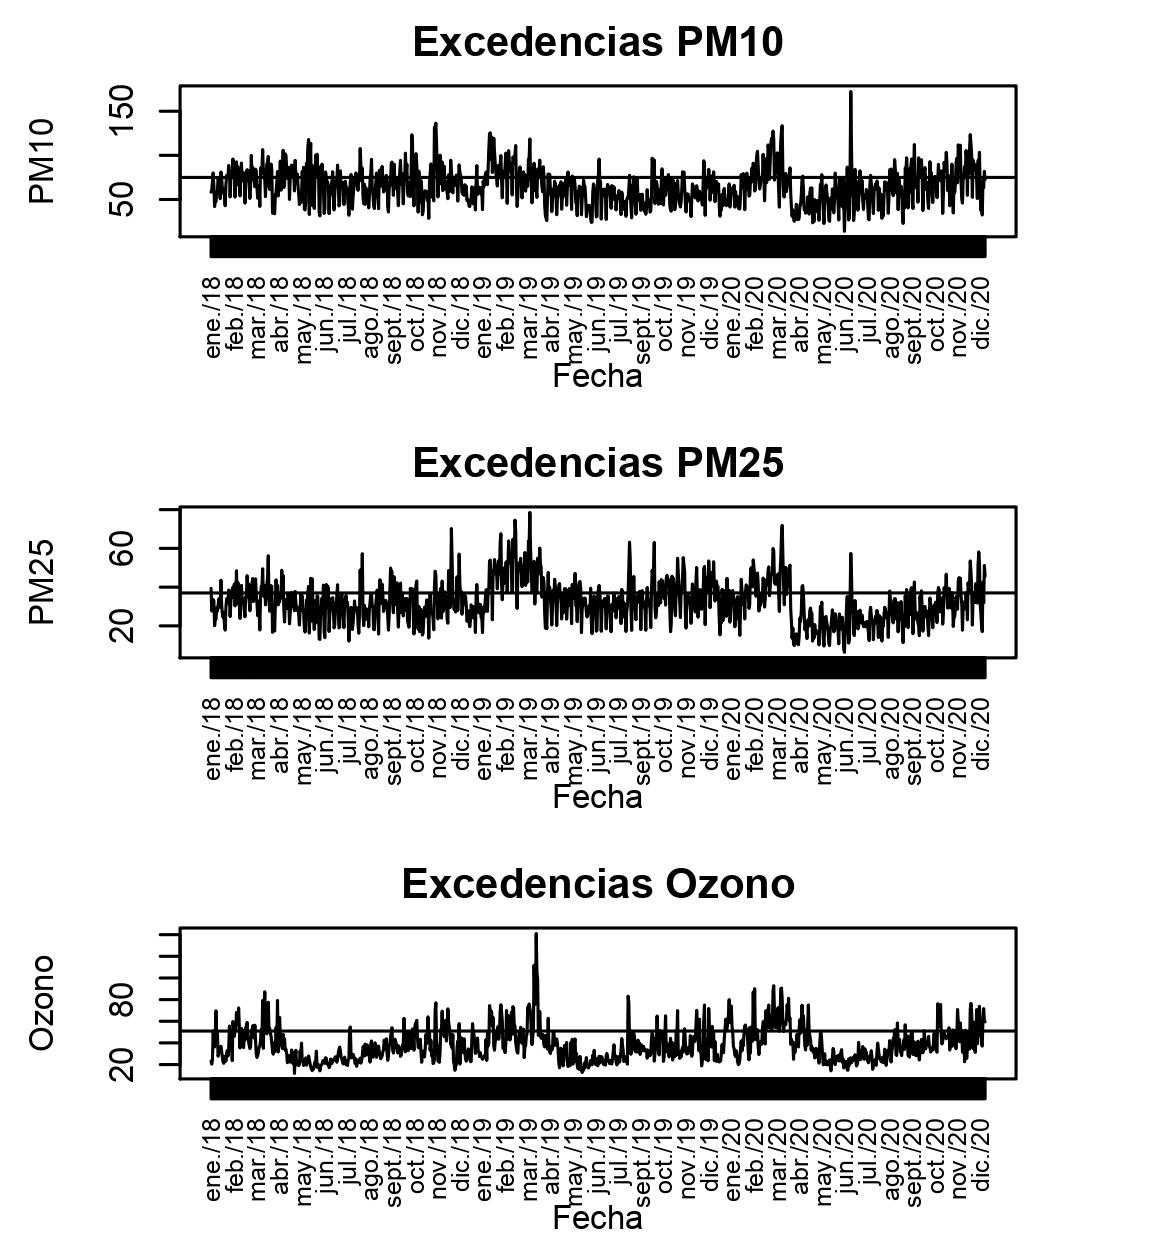
\includegraphics[scale=1.5]{seriesdetiempo}
\end{center}
\centering
\caption{Niveles de concentración diaria de contaminantes $O_3$, $PM_{10}$ y $PM_{2.5}$, la recta horizontal representa el umbral máximo permitido por las autoridades ambientales en Colombia.}
\label{seriesdet}
\end{figure}

En la tabla \ref{rebasesporcontaminante} se muestra un resumen de los rebases obtenidos para cada uno de los contaminantes de interés, teniendo en cuenta que para el $O_3$ los rebases se determinaron sobre un valor de $50.93$ luego de realizar la respectiva conversión de partes por billón a $\mu g/m^3$. 

En la figura \ref{mediasacum} se presentan los graficos de las medias acumuladas de los rebases de los umbrales máximos permitidos. En ellos se puede evidenciar que hubo meses en los cuales no se presentaron rebases, esto se observa cuando las gráficas se muestran como una constante, un ejemplo es el caso del Ozono, en los meses comprendidos entre marzo y julio de 2018, no hubo ni un solo rebase, así como también entre los meses de abril y agosto del año 2019. De esta misma manera ocurre con los otros dos contaminantes, sin embargo es el Ozono, en el cual los periodos en los que no se rebasan los umbrales son mas extensos. 



\begin{table}[!h]
\begin{center}
\begin{tabular}{|c|c|c|c|}
\hline
Contaminante & Umbral & Rebases & Porcentaje \\
\hline \hline
$PM_{10}$ & $70\mu g /m^3$ &  318  & $29\%$ \\ \hline
$0_3$& $100 ppb$ &  219 & $20\%$  \\ \hline
$PM_{2.5}$ & $37\mu g /m^3$ & 332 & $30.3 \%$  \\ \hline
\end{tabular}
\caption{Número de rebases de cada contaminante.}
\label{rebasesporcontaminante}
\end{center}
\end{table}


 
\begin{figure}[!t]
\begin{center}
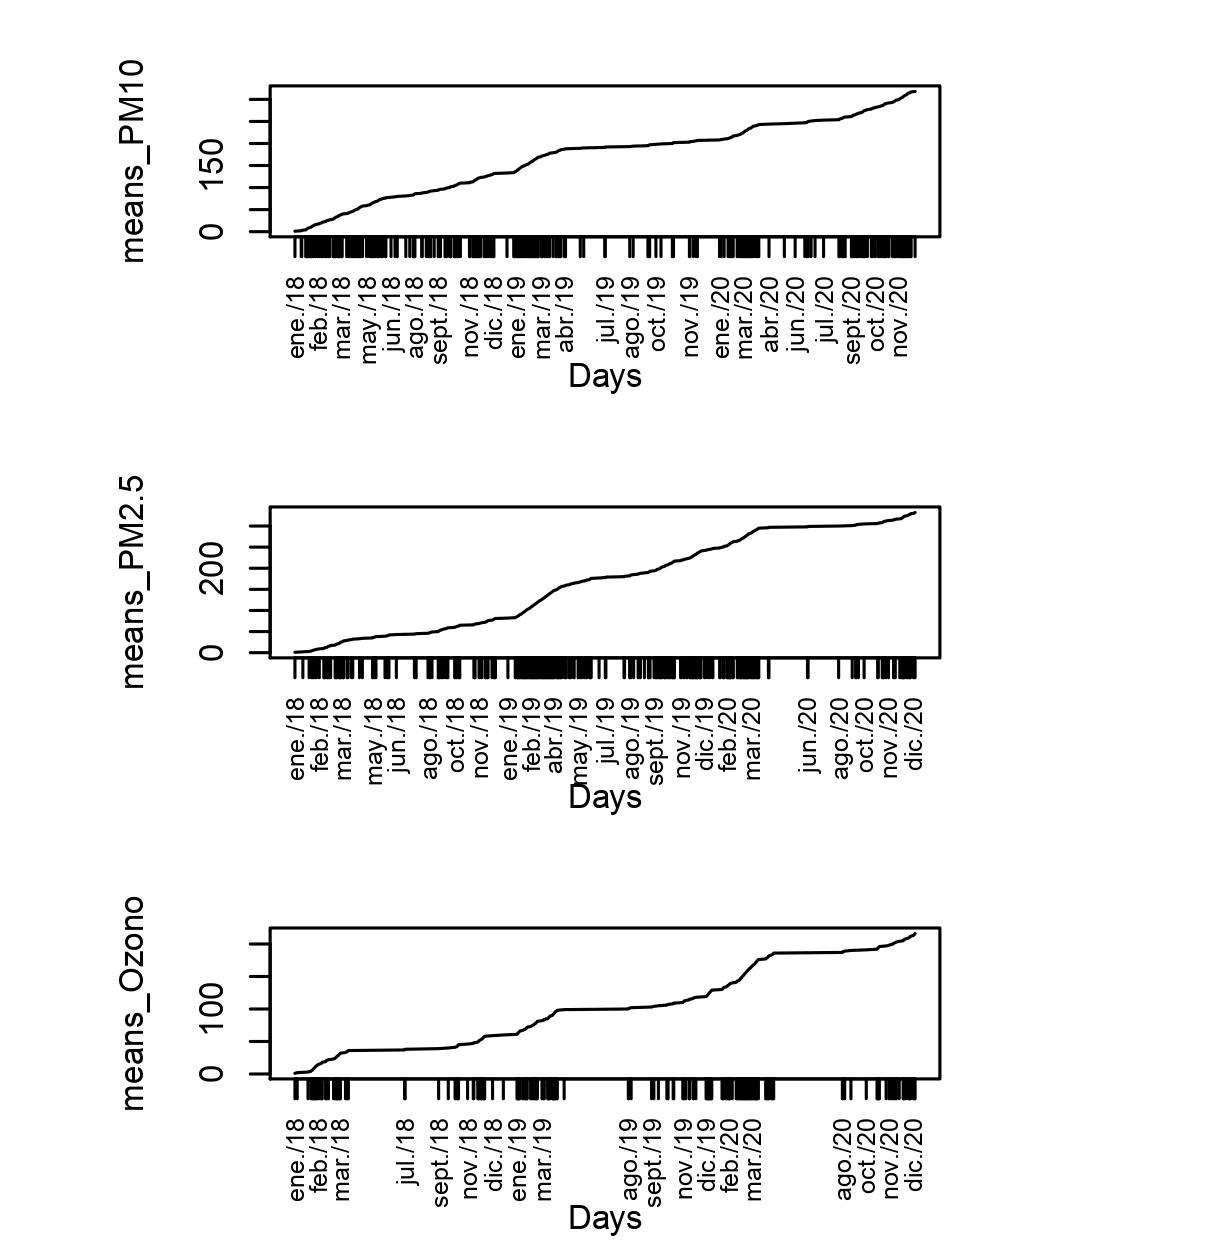
\includegraphics[scale=1.5]{mediasacumuladas}
\end{center}
\centering
\caption{Media acumulada observada del número de excedencias para cada uno de los tres contaminantes.}
\label{mediasacum}
\end{figure}

Para estudiar el número de rebases de los umbrales ambientales, se considera un proceso de Poisson con función de intensidad $\lambda (t),$ con la forma Weibull, que depende de los parámetros $\a$ y $\b$ de acuerdo con la siguiente expresión: 

$$\lambda(t)=\frac{\a}{\b}\left(\frac{t}{\b}   \right)^{\a -1}, \a, \b >0 \text{ y } t \geq 0 $$ 

A partir de esta expresión se construyen las funciones de riesgo para cada uno de los modelos, teniendo en cuenta que cuando el parámetro $\a<1$ la función es decreciente, si $\a>1$  será creciente y constante cuando $\a=1$

\section{Sin puntos de cambio}

Para estimar los parámetros de este modelo, se realizaron $20.000$ iteraciones y se eliminaron $2.000$ de ellas. En esta implementación se encontró que para el $PM_{10}$, los parámetros son $\a=1.02$ y $\b=3.87$, lo cual indica que la función de riesgo será creciente, esto lo que quiere decir, es que el número de rebases tiende a aumentar con el paso del tiempo. 

Para el caso del $PM_{2.5}$, se obtuvo: $\a=1.16$ y $\b=1.75$ y para el ozono, $\a=1.21$ y $\b=13.37$, estos últimos valores de $\a$ demuestran que las funciones también son crecientes, de manera que con el paso del tiempo los niveles de contaminación de $PM_{2.5}$ y $O_3$ aumentarán.  

En ausencia de puntos de cambio, se determinaron los siguientes parámetros $\a$  y  $\b$ con los cuales se podrán construir las funciones de riesgo acumuladas: 

\begin{table}[!h]
\centering
\begin{tabular}{|l|l|l|l|l|l|}
\hline
& \multicolumn{5}{c|}{Información estadística} \\
\cline{2-6}
& Parámetros & dist. inicial  & Media & sd  &   intervalo $95 \%$\\
\hline \hline
\multirow{2}{1.5cm}{$PM_{10}$} & $\a_1$ & $unif(1,3)$ & $1.02$ & $0.01$ & $(1.00;1.06)$ \\ \cline{2-6}
& $\b_1$& $unif(1,10)$ & $3.87$ & $0.45$ & $(3.25;4.99)$\\  \cline{1-6}
\multirow{2}{1.5cm}{$PM_{2.5}$} & $\a_1$ & $dunif(1,2.5)$& $1.16$ & $0.03$ & $(1.12;1.24)$\\ \cline{2-6}
& $\b_1$ & \multicolumn{1}{c|}{$dunif(6.3;78.5)$} & $1.75$ & $0.42$ & $(6.43;10.13)$\\ \cline{1-6}
\multirow{2}{1.5cm}{$O_3$} & $\a_1$ & $dunif(1,5.99)$ & $1.21$& $0.03$ & $(1.16;1.29)$\\ \cline{2-6}
&$\b_1$ & \multicolumn{1}{c|}{$dunif(11.9,141)$} & $13.37$ & $1.41$ & $(11.94;17.12)$\\ \cline{1-6}
\end{tabular}
\caption{Información estadística de cada modelo sin puntos de cambio.}
\label{infoestad}
\end{table}



Teniendo estos parámetros,en la figura \ref{riesgo} se presentan las diferentes funciones de riesgo $\lambda (t)$ para cada uno de los tres contaminantes, esto sin tener en cuenta algún punto de cambio. 



\begin{figure}[!h]
\begin{center}
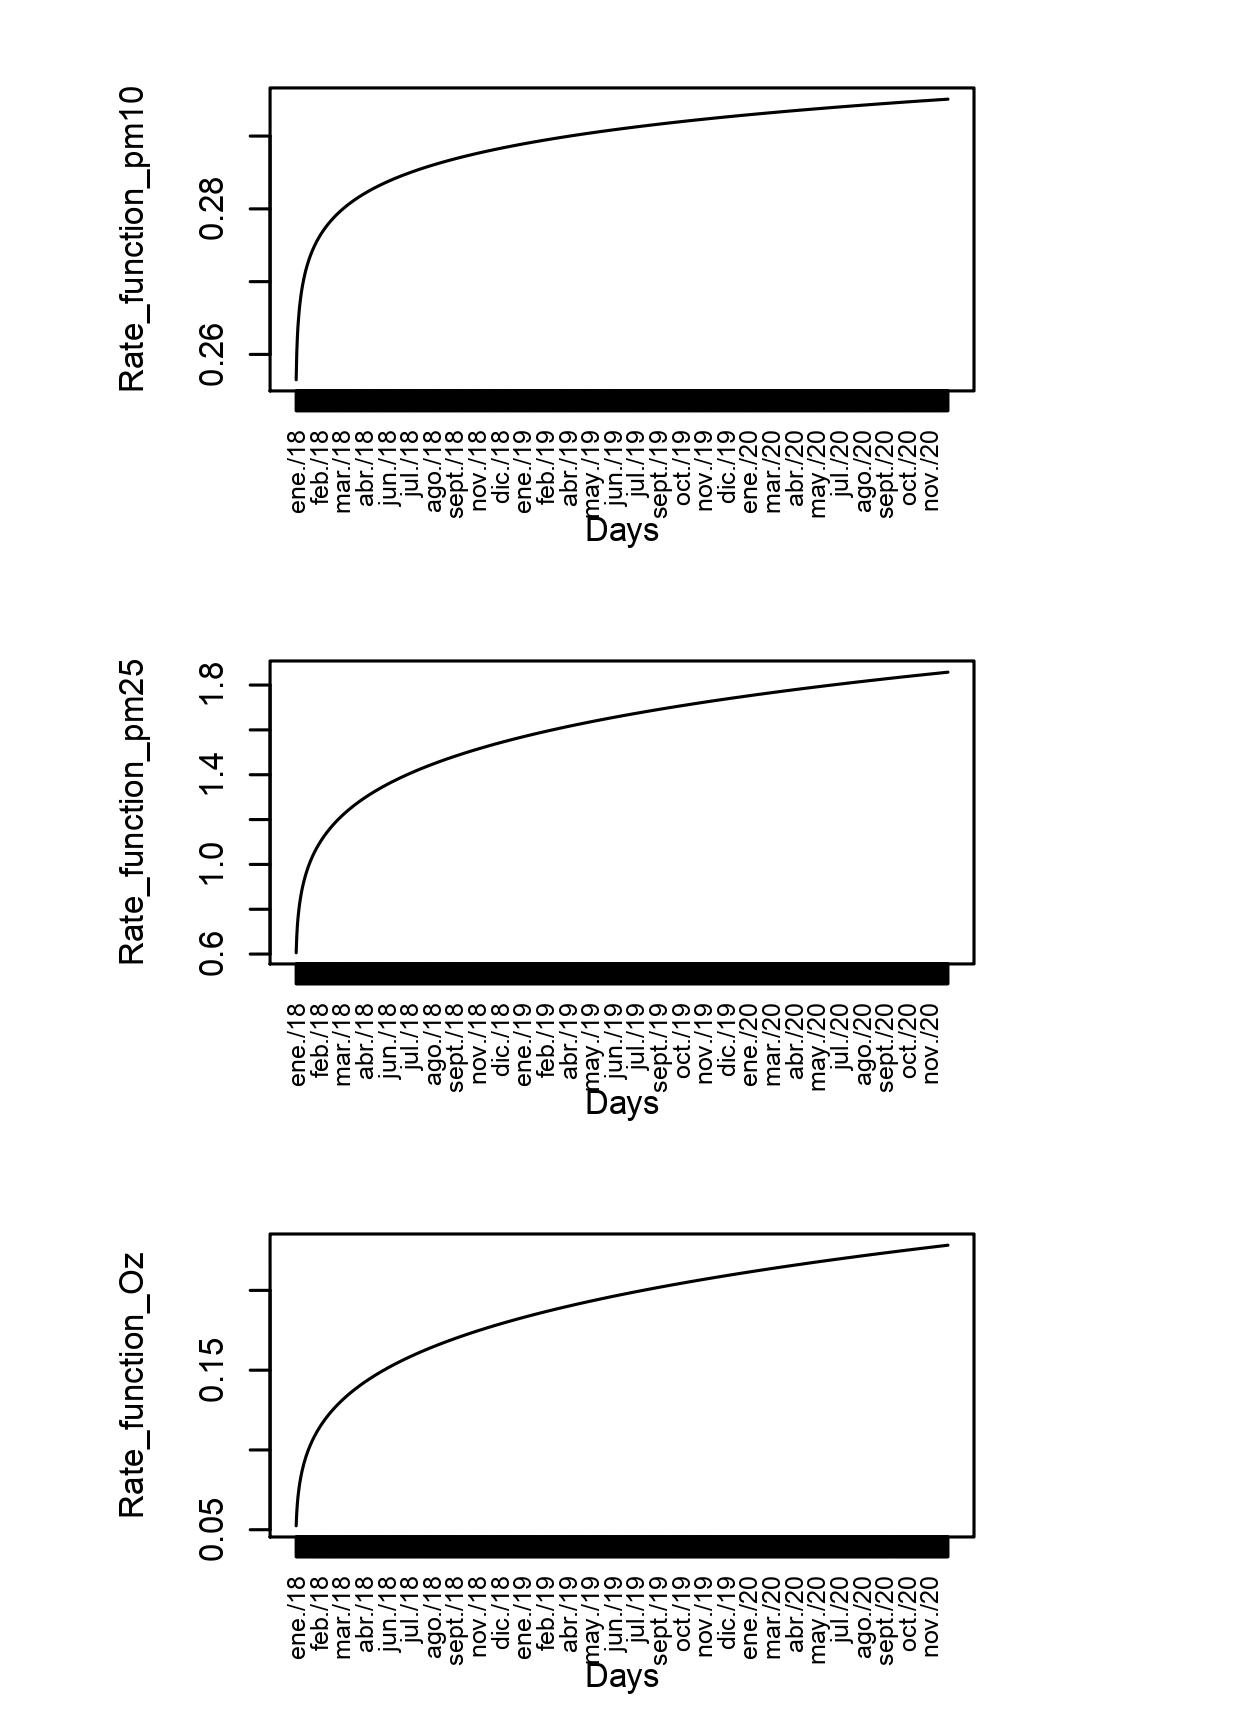
\includegraphics[width=15cm]{rate_function_spdc}
\end{center}
\centering
\caption{ Función de riesgo $\lambda (t) $, estimada para el modelo en ausencia de puntos de cambio.  }
\label{riesgo}
\end{figure}


El comportamiento de los rebases de cada contaminante se puede observar a través de la función de media acumulada $m(t)$, observada y estimada. En nuestro caso se observa en la figura  \ref{mediasacumcomp}, la función de media acumulada estimada en color azul, frente a lo estimado con un intervalo de confianza del $95\%$ de credibilidad, lo cual se representa mediante las lineas verdes, buscando hacer un ajuste y contraste con lo observado, que se presenta de color negro.



\begin{figure}[h!]
\begin{center}
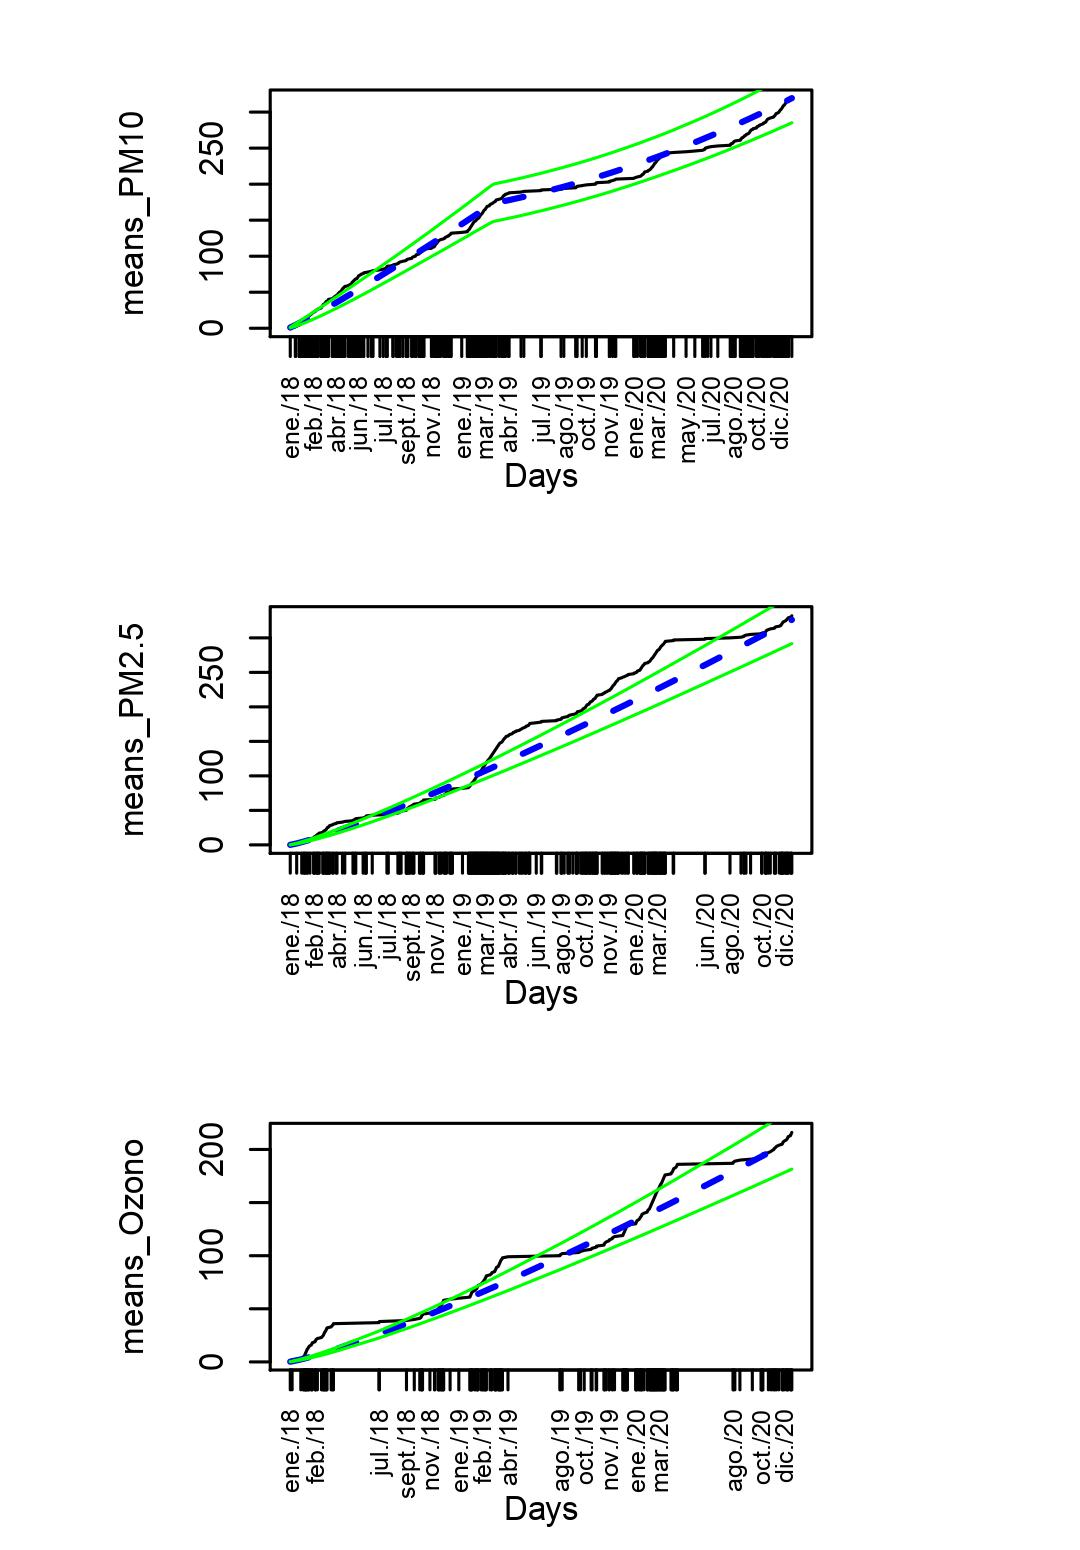
\includegraphics[width=13cm]{spdc_means}
\end{center}
\centering
\caption{ Función de media acumulada (azul), junto con los intervalos de confianza estimados con un 95\% de confianza (verde) y los datos observados (negro).  }
\label{mediasacumcomp}
\end{figure}



Se puede observar, que para el caso del $PM_{10}$, el modelo inicia con un buen ajuste, sin embargo para los meses posteriores a enero del 2019, se ve un desajuste considerable. Caso contrario el del $PM_{2.5}$ cuya estimación no es favorable en la mayoría de los meses estudiados, al igual que en el caso del ozono, en el cual se ve un buen ajuste durante los tres primeros meses y durante el mes de abril del año 2020. 



\newpage


\section{Un punto de cambio}
 

Este primer punto se encontró gráficamente, observando cambios en la figura \ref{mediasacum}, e identificando acontecimientos sucedidos en las fechas donde se observan dichos cambios. Estos puntos pueden ser aproximadamente los siguientes: 
$\tau_1=380$, $\tau_2=415$ y $\tau_3=115$, para $PM_{10}$, $PM_{2.5}$ y $O_3$ respectivamente.  



Para estos modelos se tendrán en cuenta dos tramos de las gráficas de medias acumuladas, que estarán determinados por el punto de cambio elegido. Es decir que antes de cada punto de cambio se determinarán un $\a$ y un $\b$ y para después del punto de cambio, otros $\a$ y $\b$ diferentes. Estos modelos se presentan en la figura \ref{mediasacumupc}

\begin{figure}[h!]
\begin{center}
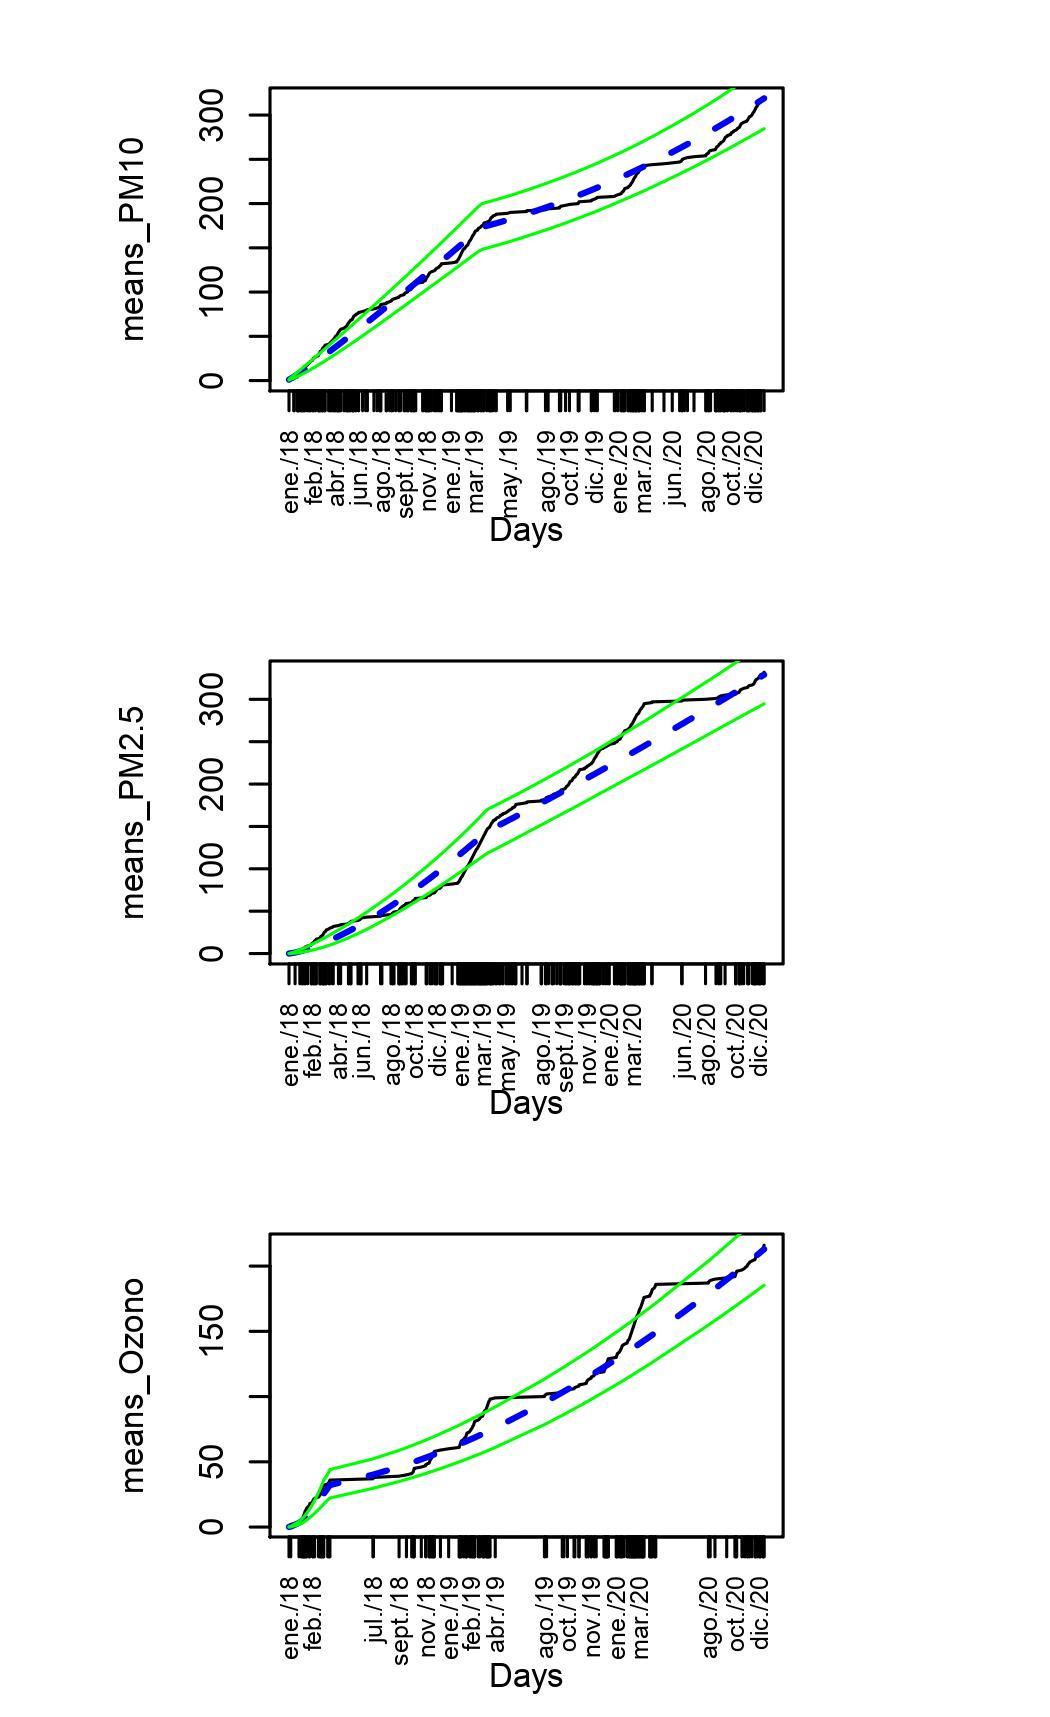
\includegraphics[width=12cm]{means_updc}
\end{center}
\centering
\caption{ Función de media acumulada (azul), junto con los intervalos de confianza estimados con un 95\% de confianza (verde) y los datos observados (negro), para un punto de cambio.  }
\label{mediasacumupc}
\end{figure}


Los parámetros estimados para este modelo, fueron obtenidos realizando 20.000 iteraciones, al igual que en sin un punto de cambio. Se observa aquí que los parámetros $\a$ para el contaminante $PM_{10}$ fueron mayores que $1$, lo que indica que el comportamiento del contaminante, tiende a  aumentar su concentración con el paso del tiempo. De la misma forma, para los contaminantes  $PM_{2.5}$ y $O_3$ ambos parámetros son mayores que $1$, de manera que, así como se observó en el modelo sin puntos de cambio, antes y después del punto establecido, los contaminantes mantienen la predicción de aumento con el paso del tiempo. Estos resultados se encuentran resumidos en la tabla \ref{infoestadupc} y la gráfica correspondiente a las funciones de riesgo se muestran en la figura 
 


\begin{table}[!h]
\centering
\begin{tabular}{|l|c|l|l|l|l|}
\hline
& \multicolumn{5}{c|}{Información estadística} \\
\cline{2-6}
& Parámetros & dist. inicial  & Media & sd  &   intervalo $95 \%$\\
\hline \hline
\multirow{5}{1.5cm}{$PM_{10}$} & $\tau_1$ & $dunif(350,450))$ & $318.94$ & $ 17.86 $ & $(284.70;354.50)$ \\ \cline{2-6}
& $\a_1$& $dunif(1, 3)$ & $1.09$ & $0.06$ & $(1.00;1.23)$\\  \cline{2-6}
& $\b_1$& $dunif(1,100)$ & $316.30$ & $17.61$ & $(282.86;351.89)$\\  \cline{2-6}
& $\a_2$& $dunif(1,3)$ & $2.02$ & $0.11$ & $(1.74; 2.17)$\\  \cline{2-6}
& $\b_2$& $dunif(1,100)$ & $316.61$ & $17.63 $ & $(283.16;352.24)$\\  \cline{1-6}
\multirow{5}{1.5cm}{$PM_{2.5}$} & $\tau_1$ & $dunif(350,500)$& $483.53$ & $9.44$ & $(465.86;498.37)$\\ \cline{2-6}
& $\a_1$& $dunif(1,2.5)$ & $1.45$ & $0.11$ & $(1.25;1.68)$\\  \cline{2-6}
& $\b_1$& $dunif(6.4, 78.5)$ & $14.90$ & $4.04$ & $(8.19;23.72)$\\  \cline{2-6}
& $\a_2$& $dunif(1,2.5))$ & $1.28$ & $0.15$ & $(1.10;1.65)$\\  \cline{2-6}
& $\b_2$& $dunif(6.4, 78.5)$ & $15.21$ & $9.15$ & $(6.58;41.13)$\\  \cline{1-6}
\multirow{5}{1.5cm}{$O_3$} & $\tau_1$ & $dunif(50,200)$ & $49.70$& $14.52$ & $(23.24;82.00)$\\ \cline{2-6}
& $\a_1$& $dunif(1, 5.9)$ & $1.83$ & $0.17$ & $(1.57;2.24)$\\  \cline{2-6}
& $\b_1$& $dunif(11.9, 141)$ & $212.85$ & $14.48$ & $(185.59;242.55)$\\  \cline{2-6}
& $\a_2$& $dunif(1, 5.9)$ & $1.67$ & $0.16$ & $(1.36;2.00)$\\  \cline{2-6}
& $\b_2$& $dunif(11.9, 141)$ & $14.59$ & $2.29$ & $(11.98;20.36)$\\  \cline{1-6}
\end{tabular}
\caption{Información estadística de cada modelo con un  punto de cambio.}
\label{infoestadupc}
\end{table}


\begin{figure}[hbt!]
\begin{center}
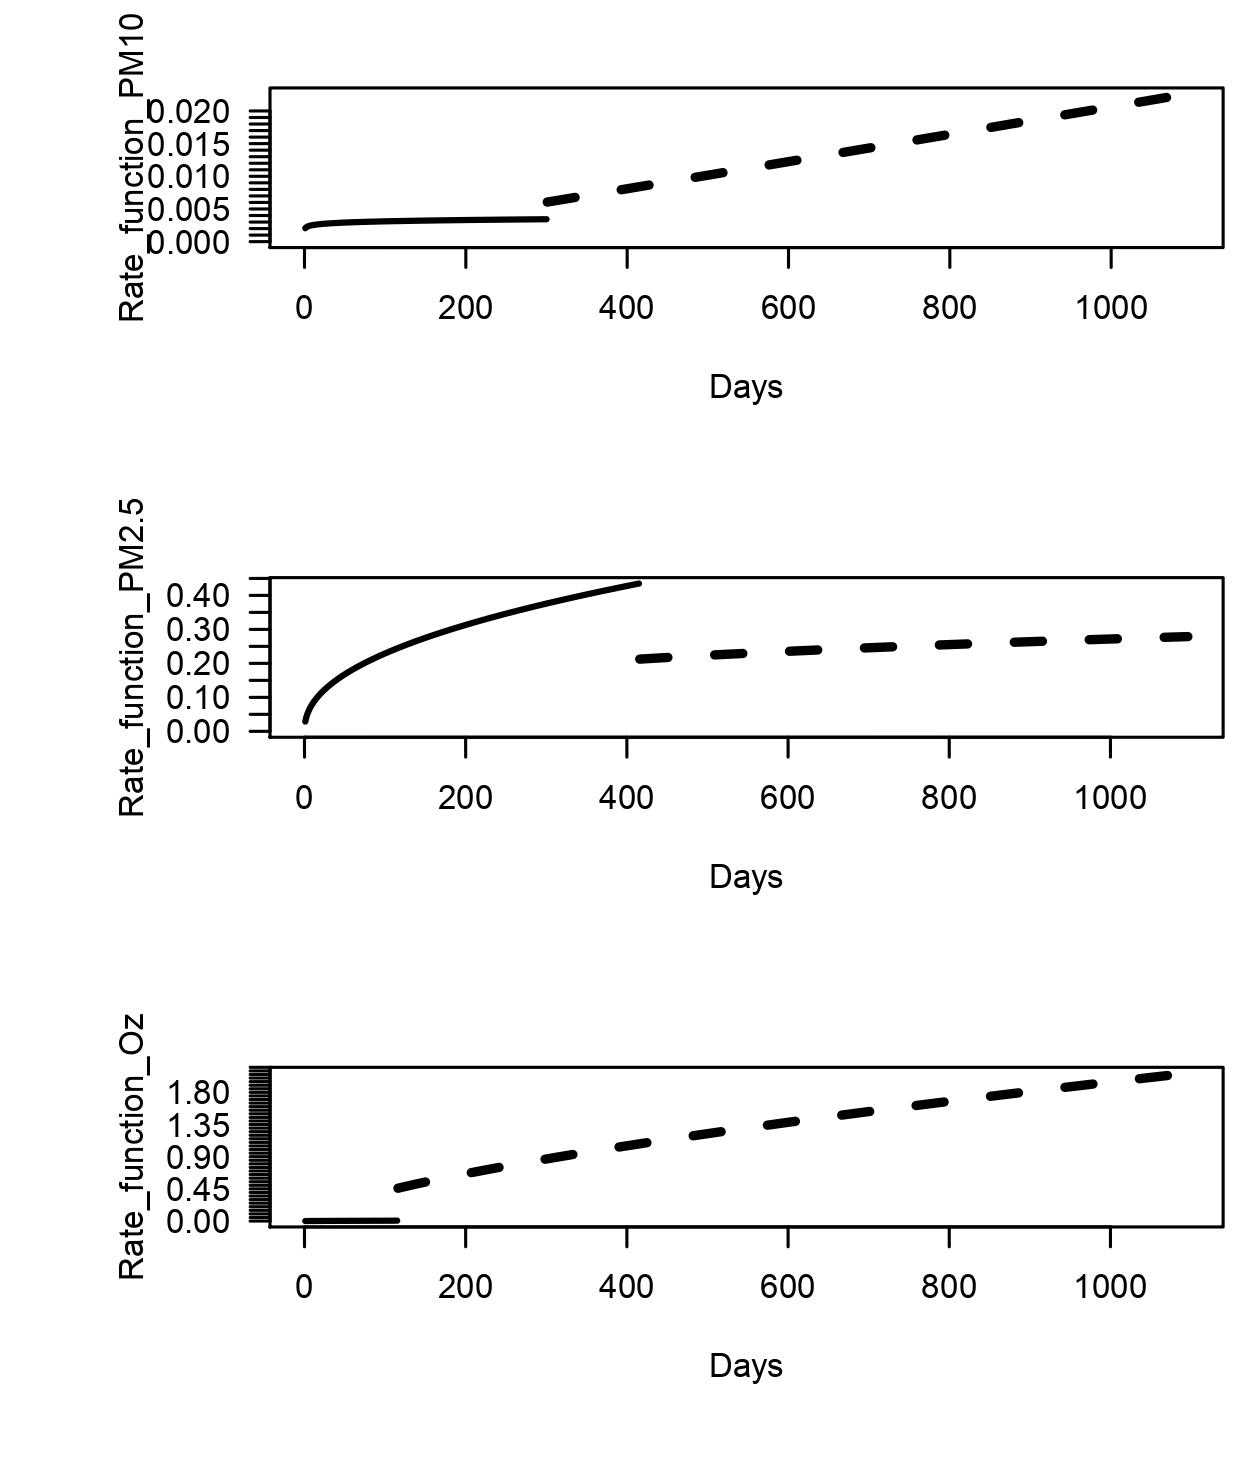
\includegraphics[width=13cm]{Rate_function_upc}
\end{center}
\centering
\caption{ Función de riesgo $\lambda (t)$, estimada para el modelo construido bajo un punto de cambio.   }
\label{rate_upc}
\end{figure}


\section{Dos puntos de cambio:}

\section{Política pública:}

Como ya se mencionó, los puntos de cambio de los modelos construidos se determinaron principalmente con ayuda de las gráficas de las medias acumuladas de cada uno de los contaminantes, para justificar estos puntos, una estrategia es identificar algunas de las estrategias del gobierno nacional para mitigar la contaminación ambiental durante estas fechas.
Uno de los insumos mas importantes que permite identificar esto, es el \textit{plan decenal de desconaminación del aire de Bogotá} que elabora cada 10 años y al cual se le realizan revisiones periódicas para verificar su alcance y cumplimiento. 
El documento que compete a esta investigación, es el elaborado para la década del 2010 al 2020 \cite{plandecenal}, en el cual, al igual que en la anterior década, se centran en la implementación de las siguientes acciones para mejorar la calidad del aire 

\begin{itemize}
\item Pico y placa ambiental.
\item Pico y placa de movilidad. 
\item Mejoramiento del ACPM.
\item Operativos en Vía.
\item Control a fuentes industriales.
\item Inventarios de emisiones. 
\end{itemize}

Estas acciones, se organizaron para ser implementadas durante los 10 años, para el caso del periodo de tiempo que se esta teniendo en cuenta en el presente documento, las acciones planteadas son, para el 2019 y 2020 únicamente, en el sector industrial, se estableció el proyecto \textit{Uso de sistemas de control
de emisiones}, para los años 2012 al 2020, en cuestiones de transporte, se debían implementar los proyectos \textit{Uso de sistemas de control de emisiones en vehículos de transporte de carga}, y \textit{Uso de sistemas de control 
de emisiones en motocicletas} y para el periodo comprendido entre 2011 y 2020 el proyecto \textit{Implementación del sistema
integrado de transporte
público}. 
Buscando que, de acuerdo con las proyecciones y con los proyectos establecidos, la tendencia de contaminación del material particulado, por ejemplo, muestre el comportamiento mostrado en la figura \ref{proyeccionplandecenal}

\begin{figure}[hbt!]
\begin{center}
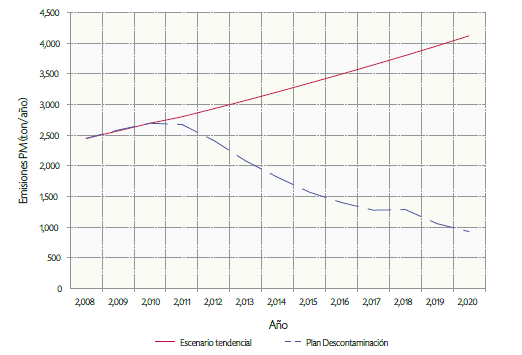
\includegraphics[width=13cm]{proyeccionplandecenal}
\end{center}
\centering
\caption{ Emisiones de material particulado entre 2008 y 2020, en los escenarios de tendencia versus el plan de descontaminación, tomado del plan decenal de descontaminación del aire de Bogotá \cite{plandecenal}. }
\label{proyeccionplandecenal}
\end{figure}

En la ciudad de Bogotá, se han reducido los niveles de concentración de $PM_{10}$ y $PM_{2.5}$ entre los años de 2012 y 2017 gracias a las propuestas implementadas en el plan decenal de decontaminación del aire para Bogotá, como por ejemplo la integración del transporte público SITP y la descontinuación de algunas busetas que no cumplían con las características establecidas para contrarrestar la contaminación; el seguimiento y control en la industria, aumento en los días sin carro, entre otras.
Puntualmente, para el caso del $PM_{10}$ y el $PM_{2.5}$ su primer punto de cambio ocurre al rededor del dato 400, el cual corresponde a una fecha aproximada al 4 de febrero del 2019, este cambio se puede explicar en parte, por la resolución 383 del año 2019 \cite{res2019}, en la cual se declara alerta amarilla porque el material particulado excede los umbrales máximos permitidos. Así mismo, para el caso del Ozono, sucede algo similar solo que su primer punto de cambio ocurre en marzo del 2018, cuando en la resolución 831 de 2018 \cite{res2018} también es decretada la alerta amarilla por contaminación ambiental y se establecen algunas restricciones en la ciudad de Bogotá, como por ejemplo establecer  restricciones en el sector de transporte y movilidad y restringir la operaciones de fuentes fijas industriales que operan con combustibles sólidos y líquidos. 

 


\section{Diagnóstico de convergencias}

\subsection{Sin puntos de cambio}
De acuerdo a las simulaciones generadas para cada modelo, se realizaron los análisis de convergencia correspondientes obteniendo resultados favorables que indican que el modelo muestra buenos resultados pues los parámetros cumplen la mayoría de los criterios, esto se muestra en las tablas \ref{converpm10spc}, \ref{converpm25spc} y 
\ref{converozono}. 

En todos los casos, para el criterio de convergencia propuesto en Geweke (1992), se observa que cada una de las pruebas aplicadas a las cinco cadenas realizadas, satisface la condición de que el valor $Z$ calculado, se encuentre entre el intervalo $(-2,2)$ esto da un buen indicio sobre la convergencia de los parámetros. 

Por otra parte, el criterio Heidelberg-Welch de estacionalidad fue  satisfactoria para todas las cadenas, por lo cual se identifica si el ancho medio para cada una de ellas es menor que $\varepsilon =0.1 $, y esto, en efecto es cierto en todas las cadenas realizadas para los tres contaminantes. 

Y finalmente el criterio de Gelman Rubin, menciona que valores cercanos a 1, indicarían una posible convergencia y en cada uno de los tres contaminantes su valor fue cercano a 1. De esta manera, cumpliendo la mayoría de condiciones de cada uno de los criterios de convergencia estudiados, se puede afirmar con seguridad que los parámetros estimados  funcionan adecuadamente. 


%%SPC-CONVERGENCIA-PM10

\begin{table}[!h]
\centering
\begin{tabular}{|l|c|l|l|l|l|l|}
\hline
& \multicolumn{6}{|c|}{Diagnóstico de convergencia} \\
\cline{2-7}
& Parámetro & cadena 1  & cadena 2  & cadena 3 & cadena 4 & cadena 5	 \\
\hline \hline
\multirow{2}{2.5cm}{Geweke} & $\a$ & $0.7131$ & $-0.18966$ & $0.5049$ & $-0.3310$  & $-0.3435$\\ \cline{2-7}
& $\s$& $0.7133$ & $-0.05731$ & $0.4922$ & $-0.4261$ & $-0.3172$\\
  \cline{1-7}
\multirow{2}{2.5cm}{Raftery - Lewis} & $\a$ & $1.35$& $ 1.28$ & $2.07$ & $1.26 $ & $  1.31 $\\ \cline{2-7}
& $\s$ & \multicolumn{1}{l|}{$1.51$} & $2.61$ & $1.70$ & $2.38 $ & $1.58$ \\ \cline{1-7}
\multirow{2}{2.5cm}{H-W Estacionalidad} & $\a$ & $0.877$ & $0.642$ & $0.903$ & $0.916$ & $0.680$ \\ \cline{2-7}
&$\s$ & \multicolumn{1}{l|}{$0.890$} & $0.598$ &  $ 0.826$ & $0.984$ & $0.747 $ \\ \cline{1-7}
\multirow{2}{2.5cm}{H-W $1/2$ Ancho} & $\a$ & $0.00107$ & $ 0.00106$ & $ 0.00112$ & $0.000986 $  & $ 0.000891  $  \\ \cline{2-7}
&$\s$ & \multicolumn{1}{l|}{$0.02705  $} & $0.02698$ & $0.02746  $ & $0.024899$ & $0.022256$ \\ \cline{1-7}

\multirow{2}{2.5cm}{Gelman - Rubin} & $\a$ & \multicolumn{5}{|c|}{1.00}\\ \cline{2-7}
&$\s$ &  \multicolumn{5}{|c|}{1.00} \\ \cline{1-7}



\end{tabular}
\caption{Información de convergencia para el modelo $PM_{10}$, sin puntos de cambio. H-W=Heidelberger-Welch}

\label{converpm10spc}
\end{table}





%%SPC-CONVERGENCIA-PM25

\begin{table}[!h]
\centering
\begin{tabular}{|l|c|l|l|l|l|l|}
\hline
& \multicolumn{6}{|c|}{Diagnóstico de convergencia} \\
\cline{2-7}
& Parámetro & cadena 1  & cadena 2  & cadena 3 & cadena 4 & cadena 5	 \\
\hline \hline
\multirow{2}{2.5cm}{Geweke} & $\a$ & $0.0959$ & $0.5630$ & $-1.785$ & $-1.455$  & $ -0.2081$\\ \cline{2-7}
& $\s$& $0.1362$ & $0.4231$ & $-1.836$ & $-1.423 $ & $-0.1948$\\
  \cline{1-7}
\multirow{2}{2.5cm}{Raftery - Lewis} & $\a$ & $2.51 $& $  1.85$ & $2.50$ & $2.56  $ & $  2.56  $\\ \cline{2-7}
& $\s$ & \multicolumn{1}{l|}{$ 2.13$} & $2.41$ & $2.43$ & $2.29	 $ & $2.34  $ \\ \cline{1-7}
\multirow{2}{2.5cm}{H-W Estacionalidad} & $\a$ & $0.229  $ & $0.764 $ & $0.795$ & $0.484$ & $0.0534$ \\ \cline{2-7}
&$\s$ & \multicolumn{1}{l|}{$0.308 $} & $  0.507$ &  $ 0.776 $ & $ 0.474$ & $ 0.8327 $ \\ \cline{1-7}
\multirow{2}{2.5cm}{H-W $1/2$ Ancho} & $\a$ & $0.00291$ & $0.00253$ & $0.00253$ & $0.00232 $  & $0.00246 $  \\ \cline{2-7}
&$\s$ & \multicolumn{1}{l|}{$0.09838  $} & $0.08906$ & $0.08830 $ & $ 0.07683$ & $0.07932 $ \\ \cline{1-7}

\multirow{2}{2.5cm}{Gelman - Rubin} & $\a$ & \multicolumn{5}{|c|}{1}\\ \cline{2-7}
&$\s$ &  \multicolumn{5}{|c|}{1} \\ \cline{1-7}



\end{tabular}
\caption{Información de convergencia para el modelo $PM_{2.5}$, sin puntos de cambio. H-W=Heidelberger-Welch}

\label{converpm25spc}
\end{table}




%%SPC-CONVERGENCIA-Ozono

\begin{table}[!h]
\centering
\begin{tabular}{|l|c|l|l|l|l|l|}
\hline
& \multicolumn{6}{|c|}{Diagnóstico de convergencia} \\
\cline{2-7}
& Parámetro & cadena 1  & cadena 2  & cadena 3 & cadena 4 & cadena 5	 \\
\hline \hline
\multirow{2}{2.5cm}{Geweke} & $\a$ & $0.7882$ & $0.2856 $ & $0.7351$ & $0.9028$  & $ -0.07696$\\ \cline{2-7}
& $\s$& $0.7052 $ & $0.2041$ & $0.9396$ & $0.8609$ & $-0.14975$\\
  \cline{1-7}
\multirow{2}{2.5cm}{Raftery - Lewis} & $\a$ & $ 1.72  $& $  1.67$ & $ 2.40$ & $1.94 $ & $ 1.80 $\\ \cline{2-7}
& $\s$ & \multicolumn{1}{l|}{$1.31$} & $1.26$ & $ 1.34 $ & $1.22 $ & $1.25$ \\ \cline{1-7}
\multirow{2}{2.5cm}{H-W Estacionalidad} & $\a$ & $0.408$ & $0.907 $ & $0.234$ & $ 0.351$ & $0.273$ \\ \cline{2-7}
&$\s$ & \multicolumn{1}{l|}{$0.4185$} & $ 0.924$ &  $ 0.113  $ & $0.374$ & $ 0.335  $ \\ \cline{1-7}
\multirow{2}{2.5cm}{H-W $1/2$ Ancho} & $\a$ & $0.00139$ & $0.00172$ & $0.00163$ & $0.0018 $  & $0.00151$  \\ \cline{2-7}
&$\s$ & \multicolumn{1}{l|}{$0.06699 $} & $0.08421$ & $0.07863$ & $ 0.0883$ & $0.07574 $ \\ \cline{1-7}

\multirow{2}{2.5cm}{Gelman - Rubin} & $\a$ & \multicolumn{5}{|c|}{1}\\ \cline{2-7}
&$\s$ &  \multicolumn{5}{|c|}{1.01} \\ \cline{1-7}



\end{tabular}
\caption{Información de convergencia para el modelo $O_3$, sin puntos de cambio. H-W=Heidelberger-Welch}
\label{converozono}
\end{table}

\subsection{Un punto de cambio}

El diagnóstico de convergencia para un punto de cambio, arrojó algunos resultados importantes que se deben mencionar. Iniciando con el criterio de Geweke (1992), este es satisfactorio en las cinco cadenas realizadas para el material particulado de $10\mu m$ de tamaño pues la comparación de los valores de las medias iniciales y finales de las cadenas, están entre -2 y 2. Para el caso del $PM_{2.5}$ se observa en la tabla \ref{convergencia_updc_pm25} que en algunas de las cadenas los valores no se encuentran entre -2 y 2, es el caso de los parámetros $\a_2$ y $\s_2$, en los cuales en dos y tres de las cadenas, respectivamente, los resultados se encuentran fuera del intervalo que se considera adecuado, sin embargo, estos números no son significativamente grandes. Para el caso del $O_3$ sucede lo mismo que en el $PM_{10}$ pues todos sus valores se encuentran dentro del intervalo que genera confianza, para poder hablar de estacionalidad y posiblemente de convergencia. 

Otro de los criterios que proporciona información sobre la convergencia de los parámetros es el test de estacionalidad de Heidelberger-Welch, pues los tres contaminantes lo pasaron, de manera que se procede a hacer la revisión del criterio del Ancho medio, el cual es satisfactorio para todos los parámetros $\a_1$ y $\a_2$ de los tres contaminantes, a excepción de una cadena del contaminante Ozono, sin embargo al ser solo una de cinco cadenas, no se tiene en cuenta, de forma que todos los parámetros $a_1$ y $a_2$ tienen una confirmación más de que tienen convergencia. Para el caso de los parámetros $\s_1$ y $\s_2$ este criterio, muestra que en algunas cadenas, sus valores no son menores a $0.1$, por tanto este criterio no es suficiente o de apoyo para argumentar convergencia de ellos, de forma similar con el parámetro $\tau$ en el caso de los tres contaminantes. 


Finalmente, para el caso de los modelos con un solo punto de cambio, se observó que el criterio Gelman- Rubin, es satisfactorio en los tres modelos, pues sus valores son cercanos a 1, toda la información anterior, se encuentra resumida en las tablas \ref{convergencia_updc_pm10}, \ref{convergencia_updc_pm25} y \ref{convergencia_updc_ozono}.


%%%%%TABLA DE CONV UPDC PM10


\begin{table}[!h]
\centering
\begin{tabular}{|l|c|l|l|l|l|l|}
\hline
& \multicolumn{6}{|c|}{Diagnóstico de convergencia} \\
\cline{2-7}
& Parámetro & cadena 1  & cadena 2  & cadena 3 & cadena 4 & cadena 5	 \\
\hline \hline
\multirow{5}{2.5cm}{Geweke} & $\a_1$ & $-0.2161$ & $-0.3797$ & $0.8125 $ & $-0.6749$  & $ 1.4716$\\ \cline{2-7}
& $\s_1$& $-0.2583 $ & $-0.3447$ & $0.8189$ & $-0.6263$ & $ 1.5856$\\
\cline{2-7}
& $\a_2$& $-0.3066 $ & $-0.1314 $ & $-1.1402$ & $ -0.4315$ & $1.0628$\\
\cline{2-7}
& $\s_2$& $-0.3165 $ & $0.1059$ & $-1.1862$ & $ -0.4369$ & $1.0672$\\
\cline{2-7}
& $\tau $& $-1.8701 $ & $-0.6091$ & $-1.4073$ & $0.1858$ & $-0.7393$\\
  \cline{1-7}
  \multirow{5}{2.5cm}{Raftery - Lewis} & $\a_1$ & $4.49$ & $5.25  $ & $2.88 $ & $2.67$  & $ 2.83 $\\ \cline{2-7}
& $\s_1$& $3.64 $ & $3.41 $ & $3.51$ & $3.01$ & $36.30 $\\
\cline{2-7}
& $\a_2$ & $18.60  $ & $30.10 $ & $13.60$ & $27.40$ & $4.69$\\
\cline{2-7}
& $\s_2$& $19.00 $ & $28.50$ & $13.80$ & $29.10 $ & $44.70$\\
\cline{2-7}
& $\tau $& $5.81 $ & $6.90$ & $6.85$ & $6.32 $ & $5.95$\\
  \cline{1-7}
  \multirow{5}{2.5cm}{H-W Estacionalidad} & $\a_1$ & $0.5609$ & $0.986 $ & $ 0.193$ & $0.186$  & $0.996$\\ \cline{2-7}
& $\s_1$& $0.5359  $ & $0.983   $ & $0.259$ & $0.212$ & $0.995$\\
\cline{2-7}
& $\a_2$& $0.0573 $ & $0.509$ & $0.651$ & $0.122$ & $0.653$\\
\cline{2-7}
& $\s_2$& $0.0973 $ & $0.593 $ & $0.639$ & $0.125$ & $0.646$\\
\cline{2-7}
& $\tau$& $0.4983 $ & $0.637 $ & $0.645$ & $0.327$ & $0.384$\\
  \cline{1-7}
  \multirow{5}{2.5cm}{H-W $1/2$ Ancho} & $\a_1$ & $0.00642$ & $0.00547 $ & $0.00679$ & $0.00705$  & $ 0.00758$\\ \cline{2-7}
& $\s_1$& $0.12170 $ & $0.10158$ & $0.12922$ & $0.13551$ & $0.14583$\\
\cline{2-7}
& $\a_2$& $0.01301 $ & $0.01932$ & $0.01404$ & $0.01324$ & $0.01780$\\
\cline{2-7}
& $\s_2$& $1.57577$ & $1.86337$ & $1.58302$ & $ 1.43715$ & $1.75334$\\
\cline{2-7}
& $\tau$& $0.16809  $ & $0.17736$ & $0.19509 $ & $0.18970$ & $0.21971$\\
  \cline{1-7}

\multirow{5}{2.5cm}{Gelman - Rubin} & $\a_1$ & \multicolumn{5}{|c|}{1.01}\\ \cline{2-7}
&$\s_1$ &  \multicolumn{5}{|c|}{1.01} \\ \cline{2-7}
&$\a_2$ &  \multicolumn{5}{|c|}{1.00} \\ \cline{2-7}
&$\s_2$ &  \multicolumn{5}{|c|}{1.00} \\ \cline{2-7}
&$\tau$ &  \multicolumn{5}{|c|}{1.00} \\ \cline{1-7}



\end{tabular}
\caption{Información de convergencia para el modelo $PM_{10}$, un punto de cambio. H-W=Heidelberger-Welch}
\label{convergencia_updc_pm10}
\end{table}


%%%%%TABLA DE CONV UPDC PM2.5


\begin{table}[!h]
\centering
\begin{tabular}{|l|c|l|l|l|l|l|}
\hline
& \multicolumn{6}{|c|}{Diagnóstico de convergencia} \\
\cline{2-7}
& Parámetro & cadena 1  & cadena 2  & cadena 3 & cadena 4 & cadena 5	 \\
\hline \hline
\multirow{5}{2.5cm}{Geweke} & $\a_1$ & $-0.2860$ & $-1.0051$ & $-17.774$ & $0.7692$  & $ -0.5075$\\ \cline{2-7}
& $\s_1$& $-0.3071 $ & $-0.9200$ & $0-12.524$ & $0.7046 $ & $ -0.5437 $\\
\cline{2-7}
& $\a_2$& $-2.6915 $ & $-3.8182 $ & $-1.997$ & $ -1.5921$ & $-1.3143 $\\
\cline{2-7}
& $\s_2$& $-2.5533$ & $-3.4243$ & $-4.756$ & $ -1.4134$ & $-1.2864$\\
\cline{2-7}
& $\tau $& $0.2518  $ & $-0.2185 $ & $-13.928$ & $0.6264$ & $1.0813$\\
  \cline{1-7}
  \multirow{5}{2.5cm}{Raftery - Lewis} & $\a_1$ & $13.60$ & $11.20  $ & $8.37  $ & $14.30$  & $  12.10 $\\ \cline{2-7}
& $\s_1$& $12.00 $ & $13.00 $ & $6.89$ & $11.40$ & $ 12.70 $\\
\cline{2-7}
& $\a_2$ & $4.54  $ & $3.14  $ & $4.19 $ & $2.85$ & $6.01 $\\
\cline{2-7}
& $\s_2$& $3.87 $ & $3.99$ & $2.60 $ & $29.10 $ & $5.17$\\
\cline{2-7}
& $\tau $& $7.59 $ & $4.33 $ & $14.40$ & $ 8.44 $ & $ 5.05$\\
  \cline{1-7}
  \multirow{5}{2.5cm}{H-W Estacionalidad} & $\a_1$ & $0.713$ & $0.2035  $ & $ 0.970$ & $0.381$  & $0.746$\\ \cline{2-7}
& $\s_1$& $0.714  $ & $0.2018  $ & $0.982$ & $0.361$ & $0.743$\\
\cline{2-7}
& $\a_2$& $0.161$ & $0.0714$ & $0.104$ & $0.445$ & $0.217$\\
\cline{2-7}
& $\s_2$& $0.203 $ & $0.1176 $ & $0.166$ & $0.647$ & $0.322$\\
\cline{2-7}
& $\tau$& $0.951 $ & $0.1457  $ & $0.989$ & $0.563$ & $0.328$\\
  \cline{1-7}
  \multirow{5}{2.5cm}{H-W $1/2$ Ancho} & $\a_1$ & $0.0161$ & $0.0150 $ & $0.0184$ & $0.0148 $  & $ 0.0167 $\\ \cline{2-7}
& $\s_1$& $0.5514 $ & $0.5158$ & $0.5726$ & $0.4953$ & $0.5719$\\
\cline{2-7}
& $\a_2$& $0.0239 $ & $0.0206$ & $0.0149$ & $0.0154$ & $0.0120$\\
\cline{2-7}
& $\s_2$& $1.4992$ & $1.1535$ & $0.8434$ & $ 0.8537$ & $0.6364$\\
\cline{2-7}
& $\tau$& $0.2058  $ & $0.1376$ & $5.0098 $ & $0.4146$ & $0.1456$\\
  \cline{1-7}

\multirow{5}{2.5cm}{Gelman - Rubin} & $\a_1$ & \multicolumn{5}{|c|}{1.03}\\ \cline{2-7}
&$\s_1$ &  \multicolumn{5}{|c|}{1.01} \\ \cline{2-7}
&$\a_2$ &  \multicolumn{5}{|c|}{1.03} \\ \cline{2-7}
&$\s_2$ &  \multicolumn{5}{|c|}{1.05} \\ \cline{2-7}
&$\tau$ &  \multicolumn{5}{|c|}{2.65} \\ \cline{1-7}



\end{tabular}
\caption{Información de convergencia para el modelo $PM_{2.5}$, un punto de cambio. H-W=Heidelberger-Welch}
\label{convergencia_updc_pm25}
\end{table}

%%%%%TABLA DE CONV UPDC OZONO 


\begin{table}[!h]
\centering
\begin{tabular}{|l|c|l|l|l|l|l|}
\hline
& \multicolumn{6}{|c|}{Diagnóstico de convergencia} \\
\cline{2-7}
& Parámetro & cadena 1  & cadena 2  & cadena 3 & cadena 4 & cadena 5	 \\
\hline \hline
\multirow{5}{2.5cm}{Geweke} & $\a_1$ & $0.1738$ & $-1.8966$ & $0.06743$ & $-3.1571$  & $-1.49105$\\ \cline{2-7}
& $\s_1$& $-0.7537$ & $-0.8614$ & $0.23790$ & $-2.5854$ & $ -1.0130 $\\
\cline{2-7}
& $\a_2$& $-1.7965$ & $-1.6817$ & $1.22712$ & $0.8546$ & $1.02269$\\
\cline{2-7}
& $\s_2$& $-1.9557$ & $-1.6606$ & $1.19464$ & $  0.8934$ & $ 0.9521$\\
\cline{2-7}
& $\tau $& $-0.7835   $ & $ 1.1726 $ & $-0.22160$ & $0.9531$ & $1.7600$\\
  \cline{1-7}
  \multirow{5}{2.5cm}{Raftery - Lewis} & $\a_1$ & $2.54$ & $2.67$ & $1.76  $ & $ 1.80$  & $  1.91 $\\ \cline{2-7}
& $\s_1$& $1.34  $ & $1.24 $ & $1.37$ & $11.40$ & $34.00$\\
\cline{2-7}
& $\a_2$ & $ 16.60 $ & $29.60  $ & $29.40 $ & $32.50$ & $ 2.51  $\\
\cline{2-7}
& $\s_2$& $20.70 $ & $ 18.50$  & $27.60$ & $35.70 $ & $42.00$\\
\cline{2-7}
& $\tau $& $2.90	$ & $ 2.52$ & $32.30$ & $ 2.11$ & $ 9.89$\\
  \cline{1-7}
  \multirow{5}{2.5cm}{H-W Estacionalidad} & $\a_1$ & $0.360$ & $0.000394 $ & $0.421$ & $0.0629$  & $0.222 $\\ \cline{2-7}
& $\s_1$& $0.193   $ & $0.070700  $ & $0.2334$ & $0.2334$ & $0.808 $\\
\cline{2-7}
& $\a_2$& $0.634 $ & $0.731613$ & $0.529$ & $0.6852$ & $0.340$\\
\cline{2-7}
& $\s_2$& $0.582 $ & $0.777112$ & $0.504$ & $ 0.6699$ & $0.286 $\\
\cline{2-7}
& $\tau$& $0.729 $ & $0.206458 $ & $0.574$ & $ 0.3733$ & $ 0.183$\\
  \cline{1-7}
  \multirow{5}{2.5cm}{H-W $1/2$ Ancho} & $\a_1$ & $0.0134$ & $NA $ & $0.00964$ & $0.0143 $  & $0.0107 $\\ \cline{2-7}
& $\s_1$& $0.1459 $ & $0.1456$ & $0.13497$ & $0.1554$ & $0.1403$\\
\cline{2-7}
& $\a_2$& $0.0283 $ & $0.0256$ & $0.02509$ & $0.0264$ & $0.0265$\\
\cline{2-7}
& $\s_2$& $2.5965$ & $2.3807$ & $2.32836$ & $ 2.3940$ & $2.4613$\\
\cline{2-7}
& $\tau$& $1.2920 $ & $2.0953$ & $0.56484 $ & $ 1.9224$ & $0.9394$\\
  \cline{1-7}

\multirow{5}{2.5cm}{Gelman - Rubin} & $\a_1$ & \multicolumn{5}{|c|}{1.01}\\ \cline{2-7}
&$\s_1$ &  \multicolumn{5}{|c|}{1.00} \\ \cline{2-7}
&$\a_2$ &  \multicolumn{5}{|c|}{1.03} \\ \cline{2-7}
&$\s_2$ &  \multicolumn{5}{|c|}{1.03} \\ \cline{2-7}
&$\tau$ &  \multicolumn{5}{|c|}{1.16} \\ \cline{1-7}



\end{tabular}
\caption{Información de convergencia para el modelo $O_3$, un punto de cambio. H-W=Heidelberger-Welch}
\label{convergencia_updc_ozono}
\end{table}







\begin{thebibliography}{X}

\bibitem{tesisbiviana} Suárez, B. M. (2020). Modelos de Poisson no homogéneos en el estudio de contaminantes en la ciudad de Bogotá, Estadística, Universidad Nacional de Colombia, Tesis de doctorado.

\bibitem{nelsen} Nelsen, R. B. (2006) An Introduction to Copulas (Springer Series in Statistics). Springer-Verlag, Berlin, Heidelberg.  

\bibitem{res2018} RES(2018). Resolución 831 Por el cual se Declara la Alerta Amarilla por contaminación atmosférica en la ciudad de Bogotá D.C. \underline{Secretaria Distrital de Ambiente.} 

\bibitem{res2019} RES(2019). RPor la cual se Declara Alerta Amarilla en la Ciudad de Bogotá D.C, y Alerta Naranja en el Sur Occidente de la Ciudad por contaminación atmosférica, y se toman otras determinaciones. \underline{Secretaria Distrital de Ambiente.} 

\bibitem{plandecenal} SDA (2010). Plan de desconaminación del aire. 


\end{thebibliography}





\end{document}






\end{document}